\documentclass{article}
\usepackage[margin=1in]{geometry}
\usepackage{problemset}
\showsolntrue

% Custom commands
\newcommand{\R}{\mathbb{R}}
\newcommand{\X}{\mathcal{X}}
\newcommand{\Y}{\mathcal{Y}}
\newcommand{\E}{\mathbb{E}}
\newcommand{\V}{\text{Var}}
\renewcommand{\P}{\mathbb{P}}

\begin{document}

\pstitle{%
    MATH 181A%
}{
    Homework 3%
}[due Saturday, January 31 at 11:59PM]

\begin{probset}

% --- Problem 1 ---
\begin{prob}
    \begin{subprobset}
    \begin{subprob}
    (\textbf{5.3.2}) The production of a nationally marketed detergent results in certain workers receiving prolonged exposures to a Bacillus subtilis enzyme. Nineteen workers were tested to determine the effects of those exposures, if any, on various respiratory functions. One such function, airflow rate, is measured by computing the ratio of a person's forced expiratory volume (FEV1) to his or her vital capacity (VC). (Vital capacity is the maximum volume of air a person can exhale after taking as deep a breath as possible; FEV1 is the maximum volume of air a person can exhale in one second.) In persons with no lung dysfunction, the "norm" for FEV1/VC ratios is 0.80. Based on the following data (175), is it believable that exposure to the Bacillus subtilis enzyme has no effect on the FEV1/VC ratio? Answer the question by constructing a 95\% confidence interval. Assume that FEV1/VC ratios are normally distributed with $\sigma = 0.09$.

    \begin{center}
        \begin{tabular}{c|c}
            Subject & FEV1/VC \\
            \hline
            RH & 0.61 \\
            WS & 0.78 \\
            RB & 0.70 \\
            RV & 0.84 \\
            MB & 0.63 \\
            EN & 0.83 \\
            DM & 0.76 \\
            WD & 0.82 \\
            WB & 0.67 \\
            FR & 0.74 \\
            RB & 0.72 \\
            PD & 0.85 \\
            BF & 0.64 \\
            EB & 0.73 \\
            JT & 0.82 \\
            PC & 0.85 \\
            PS & 0.88 \\
            RW & 0.87 \\
            RB & 0.82 \\
        \end{tabular}
    \end{center}

    \begin{soln}
        \[
            \bar{x} = \frac{1}{19}\sum_{i=1}^{19} x_i = \frac{14.56}{19} \approx 0.7663
        \]
        Since $\sigma$ is known, we use a $z$-interval. For a 95\% confidence interval, $z_{\alpha/2} = z_{0.025} = 1.96$. The 95\% confidence interval for the true mean $\mu$ is:
        \[
            \bar{x} \pm z_{\alpha/2} \cdot \frac{\sigma}{\sqrt{n}} = 0.7663 \pm 1.96 \cdot \frac{0.09}{\sqrt{19}} = (0.7258, 0.8068)
        \]
        Since the value of 0.80 falls within the confidence interval $(0.726, 0.807)$, we cannot reject the hypothesis that exposure to the Bacillus subtilis enzyme has no effect on the FEV1/VC ratio. The data is consistent with the hypothesis that the true mean equals 0.80.
    \end{soln}
    \end{subprob}

    \newpage

    \begin{subprob}
        (\textbf{5.3.10}) In 1927, the year he hit sixty home runs, Babe Ruth batted .356, having collected 192 hits in 540 official at-bats (150). Based on his performance that season, construct a 95\% confidence interval for Ruth's probability of getting a hit in a future at-bat.

        \begin{soln}
            \begin{align*}
                \hat{p} &= \frac{192}{540} \approx 0.3556 \\
                \sqrt{\frac{\hat{p}(1-\hat{p})}{n}} &= \sqrt{\frac{0.3556 \cdot 0.6444}{540}} = \sqrt{\frac{0.2292}{540}} \approx 0.0206 \\
                \hat{p} \pm z_{\alpha/2} \cdot \sqrt{\frac{\hat{p}(1-\hat{p})}{n}} &= 0.3556 \pm 1.96 \cdot 0.0206 = (0.3152, 0.3960)
            \end{align*}
            The 95\% confidence interval for Ruth's probability of getting a hit in a future at-bat is approximately $(0.315, 0.396)$.
        \end{soln}
    \end{subprob}
    \end{subprobset}
\end{prob}

% --- Problem 2 ---
\begin{prob}[\textbf{5.3.26}]
    Suppose that $p$ is to be estimated by $\frac{X}{n}$ and we are willing to assume that the true $p$ will not be greater than 0.4. What is the smallest $n$ for which $\frac{X}{n}$ will have a 99\% probability of being within 0.05 of $p$?

    \begin{soln}
        We need $P(|\frac{X}{n} - p| \leq 0.05) \geq 0.99$, which is equivalent to $P(|\frac{X}{n} - p| \geq 0.05) \leq 0.01$.
        
        The estimator $\frac{X}{n}$ has mean $p$ and variance $\frac{p(1-p)}{n}$. By Chebyshev's inequality:
        \[
            P\left(\left|\frac{X}{n} - p\right| \geq 0.05\right) \leq \frac{\V(X/n)}{(0.05)^2} = \frac{p(1-p)}{n(0.05)^2} = \frac{p(1-p)}{0.0025n}
        \]
        
        We require $\frac{p(1-p)}{0.0025n} \leq 0.01$, which gives:
        \[
            n \geq \frac{p(1-p)}{0.0025 \times 0.01} = \frac{p(1-p)}{0.000025}
        \]
        
        Since $p \leq 0.4$, the maximum value of $p(1-p)$ occurs at $p = 0.4$, giving $p(1-p) = 0.4 \times 0.6 = 0.24$.
        
        Therefore:
        \[
            n \geq \frac{0.24}{0.000025} = 9600
        \]
        
        The smallest $n$ is 9600.
    \end{soln}
\end{prob}

\newpage

% --- Problem 3 ---
\begin{prob}
    Suppose $X_1, \ldots, X_n$ is a random sample from a Bernoulli($p$) distribution and the sample average is $\bar{x}_n = 0.45$, based on which we can construct a 95\% confidence interval for $p$. Now we collect more data and the sample average is around 0.48, we want to construct a 90\% confidence interval with the length being 1/3 of the 95\% one. How large should the sample size $n_{new}$ be in terms of $n$?

    \begin{soln}
        The length of a confidence interval for a Bernoulli proportion is $L = 2 \cdot z_{\alpha/2} \cdot \sqrt{\hat{p}(1-\hat{p})/n}$.
        \begin{align*}
            L_1 &= 2 \cdot 1.96 \cdot \sqrt{\frac{0.45 \cdot 0.55}{n}} = 3.92 \cdot \sqrt{\frac{0.2475}{n}} \\
            L_2 &= 2 \cdot 1.645 \cdot \sqrt{\frac{0.48 \cdot 0.52}{n_{new}}} = 3.29 \cdot \sqrt{\frac{0.2496}{n_{new}}}
        \end{align*}
        Setting $L_2 = \frac{1}{3} L_1$:
        \begin{align*}
            3.29 \cdot \sqrt{\frac{0.2496}{n_{new}}} &= \frac{1}{3} \cdot 3.92 \cdot \sqrt{\frac{0.2475}{n}} \\
            \sqrt{\frac{0.2496}{n_{new}}} &= \frac{3.92}{9.87} \cdot \sqrt{\frac{0.2475}{n}} \approx 0.3972 \cdot \sqrt{\frac{0.2475}{n}} \\
            \frac{0.2496}{n_{new}} &= (0.3972)^2 \cdot \frac{0.2475}{n} = \frac{0.0391}{n} \\
            n_{new} &= \frac{0.2496 \cdot n}{0.0391} \approx 6.38n
        \end{align*}
    \end{soln}
\end{prob}

\newpage

% --- Problem 4 ---
\begin{prob}[\textbf{5.4.6}]
    Let $Y_{\min}$ be the smallest order statistic in a random sample of size $n$ drawn from the uniform pdf, $f_Y(y; \theta) = 1/\theta, 0 \leq y \leq \theta$. Find an unbiased estimator for $\theta$ based on $Y_{\min}$.

    \begin{soln}
        For the uniform distribution on $[0, \theta]$, the cdf is $F_Y(y) = y/\theta$ for $0 \leq y \leq \theta$. Hence, the cdf, pdf, and expected value of $Y_{\min}$ are:
        \begin{align*}
            F_{Y_{\min}}(y) &= 1 - P(Y_{\min} > y) = 1 - [P(Y > y)]^n = 1 - \left(1 - \frac{y}{\theta}\right)^n \\
            f_{Y_{\min}}(y) &= \frac{d}{dy} F_{Y_{\min}}(y) = \frac{n}{\theta} \left(1 - \frac{y}{\theta}\right)^{n-1}, \quad 0 \leq y \leq \theta \\
            \E[Y_{\min}] &= \int_0^{\theta} y \cdot \frac{n}{\theta} \left(1 - \frac{y}{\theta}\right)^{n-1} dy
        \end{align*}
        
        Let $u = 1 - y/\theta$, so $y = \theta(1-u)$ and $dy = -\theta du$. When $y = 0$, $u = 1$; when $y = \theta$, $u = 0$:
        \begin{align*}
            \E[Y_{\min}] &= \int_1^0 \theta(1-u) \cdot \frac{n}{\theta} \cdot u^{n-1} \cdot (-\theta) du \\
            &= n\theta \int_0^1 (1-u) u^{n-1} du \\
            &= n\theta \int_0^1 (u^{n-1} - u^n) du \\
            &= n\theta \left[\frac{u^n}{n} - \frac{u^{n+1}}{n+1}\right]_0^1 \\
            &= n\theta \left(\frac{1}{n} - \frac{1}{n+1}\right) \\
            &= n\theta \cdot \frac{(n+1) - n}{n(n+1)} \\
            &= \frac{\theta}{n+1}
        \end{align*}
        
        Therefore, $\E[Y_{\min}] = \theta/(n+1)$, which implies $\E[(n+1)Y_{\min}] = \theta$. Hence, $(n+1)Y_{\min}$ is an unbiased estimator for $\theta$.
    \end{soln}
\end{prob}

\newpage

% --- Problem 5 ---
\begin{prob}[\textbf{5.4.9}]
    A random sample of size 2, $Y_1$ and $Y_2$, is drawn from the pdf \[f_Y(y; \theta) = 2y\theta^2, \quad 0 < y < \frac{1}{\theta}\] What must $c$ equal if the statistic $c(Y_1 + 2Y_2)$ is to be an unbiased estimator for $1/\theta$?

    \begin{soln}
        We need $\E[c(Y_1 + 2Y_2)] = 1/\theta$. Since $Y_1$ and $Y_2$ are identically distributed, $\E[Y_1] = \E[Y_2] = \E[Y]$. So first we compute $\E[Y]$:
        \begin{align*}
            \E[Y] &= \int_0^{1/\theta} y \cdot 2y\theta^2 dy = 2\theta^2 \int_0^{1/\theta} y^2 dy \\
            &= 2\theta^2 \left[\frac{y^3}{3}\right]_0^{1/\theta} = 2\theta^2 \cdot \frac{1}{3\theta^3} = \frac{2}{3\theta}
        \end{align*}
        
        Now, for the estimator to be unbiased, we have:
        \begin{align*}
            \E[c(Y_1 + 2Y_2)] &= c(\E[Y_1] + 2\E[Y_2]) = c(\E[Y] + 2\E[Y]) = 3c\E[Y] \\
            &= 3c \cdot \frac{2}{3\theta} = \frac{2c}{\theta} = \frac{1}{\theta}
        \end{align*}
        
        Solving for $c$:
        \[
            \frac{2c}{\theta} = \frac{1}{\theta} \implies 2c = 1 \implies c = \frac{1}{2}
        \]
        
        Therefore we have $c = 1/2$ for the estimator to be unbiased.
    \end{soln}
\end{prob}

% --- Problem 6 ---
\begin{prob}[\textbf{5.4.12}]
    We showed in Example 5.4.4 that $\hat{\sigma}^2 = \frac{1}{n} \sum_{i=1}^n (Y_i - \bar{Y})^2$ is biased for $\sigma^2$. Suppose $\mu$ is known and does not have to be estimated by $\bar{Y}$. Show that $\hat{\sigma}^2 = \frac{1}{n} \sum_{i=1}^n (Y_i - \mu)^2$ is unbiased for $\sigma^2$.

    \begin{soln}
        We compute the expected value:
        \begin{align*}
            \E[\hat{\sigma}^2] &= \E\left[\frac{1}{n} \sum_{i=1}^n (Y_i - \mu)^2\right] \\
            &= \frac{1}{n} \sum_{i=1}^n \E[(Y_i - \mu)^2] \\
            &= \frac{1}{n} \sum_{i=1}^n \V(Y_i) \\
            &= \frac{1}{n} \sum_{i=1}^n \sigma^2 \\
            &= \frac{1}{n} \cdot n \cdot \sigma^2 = \sigma^2
        \end{align*}
        
        Therefore, $\hat{\sigma}^2 = \frac{1}{n} \sum_{i=1}^n (Y_i - \mu)^2$ is unbiased for $\sigma^2$.
    \end{soln}
\end{prob}

\newpage

% --- Problem 7 ---
\begin{prob}
    For $n = 20$, simulate a random sample of size $n$ from $N (\mu, 2^2)$, where $\mu = 1$. Note that we just use $\mu = 1$ to generate the random sample. In the problem below, $\mu$ is an unknown parameter. Mark in both plots the maximum likelihood estimate of $\mu$ from the generated random sample. Plot in different figures:

    \begin{subprobset}
    \begin{subprob}
        the likelihood function of $\mu$,

        \begin{soln}
            \begin{center}
                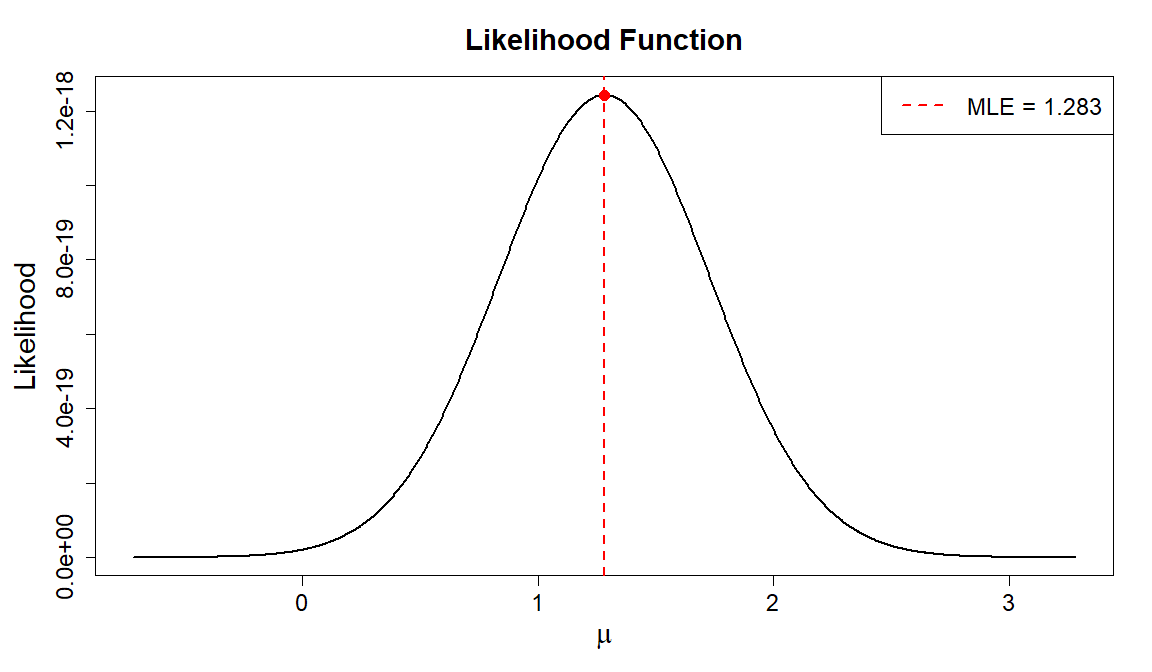
\includegraphics[width=0.8\textwidth]{Images/7.1.png}
            \end{center}
        \end{soln}
    \end{subprob}

    \begin{subprob}
        the log likelihood function of $\mu$,

        \begin{soln}
            \begin{center}
                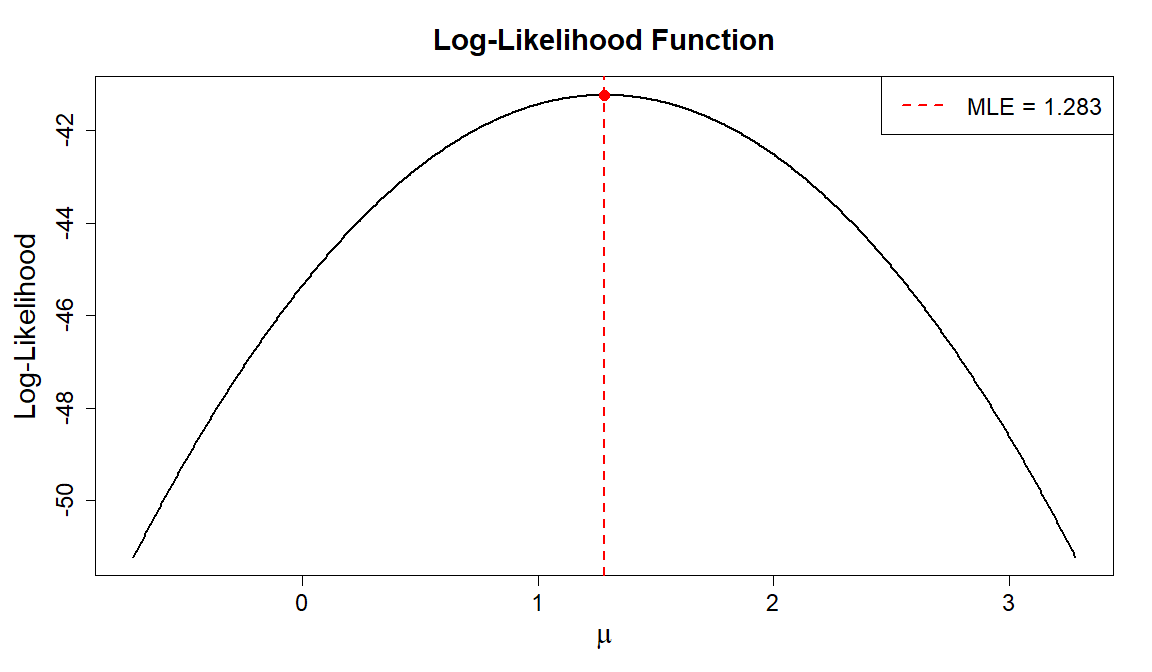
\includegraphics[width=0.8\textwidth]{Images/7.2.png}
            \end{center}
        \end{soln}
    \end{subprob}
    \end{subprobset}
\end{prob}
\end{probset}
\end{document}